\chapter{Evaluation}


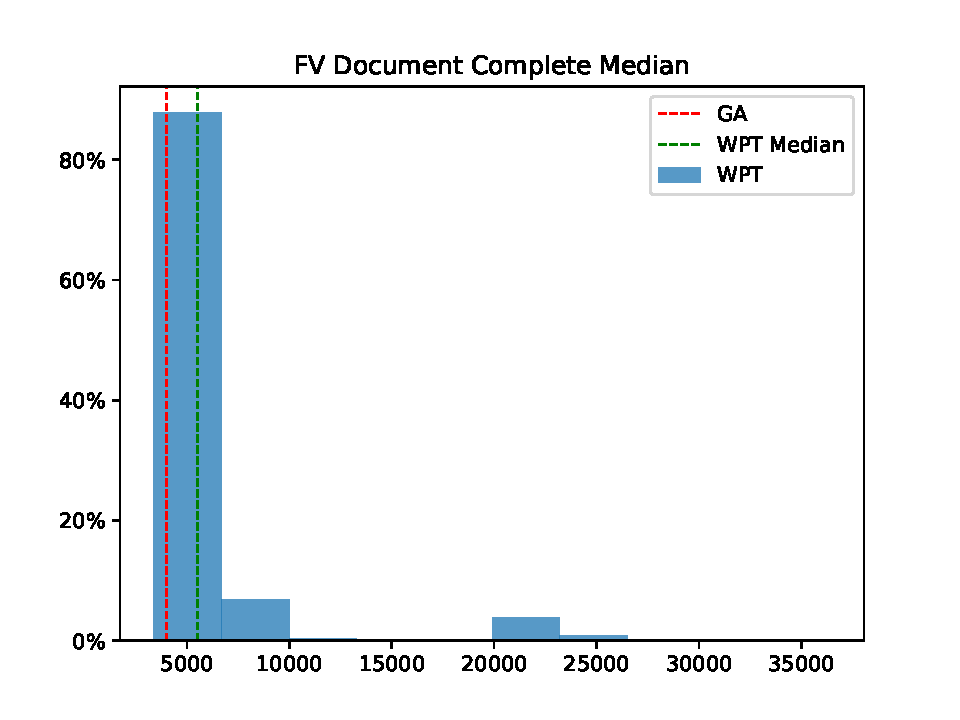
\includegraphics[width=1\textwidth]{test}


\begin{itemize}
	\item Last chapter...
	\item This chapter: Describe shortly all sections from this chapter
	\item In the next chapter...
\end{itemize}




\section{Internal, external validity}


\begin{itemize}
\item At this point, i have the data collected and can analyse it
\item The quality and quantity of the data needs to be discussed
\item Quality: There are chances that some data are malformed, e.g. because internet connection was bad, etc.
\item Quantity: Is the amount of data sufficient to make the evaluation generalisable
\end{itemize}



\section{General}

\begin{itemize}
    \item For each attempt, describe: Threats to validity, generalizability
\end{itemize}

generalizability: meine Daten zeige nur für Chrome, MacBook, diese Geschwindigkeit etc.
Und auch nur für diese Test-Website
Die Schwierigkeit der Generalisierbarkeit ist eines der grössten Probleme bei dieser Fragestellung

\section{Plain / Skeletal Website}

\begin{itemize}
\item Information gained from this experiment
\item Limitations and questions which can not be answered with this approach
\end{itemize}


\section{Mirroring}


\section{HTTP Archive inspired website}

\begin{itemize}
\item Information gained from this experiment
\item Meaning and interpretation of the collected data
\item Limitations and questions which can not be answered with this approach
\end{itemize}




\section{WebPageTest Bulk Tests}

\begin{itemize}
\item Bulk testing is a feature for private instances only
\item Misuse this feature to test the same website X times
\end{itemize}


\subsection{Bulk Test Overview: Description of test result page}

\begin{itemize}
\item Each test has Test ID: YYMMDD\textunderscore random\textunderscore random
\item Test results after bulk test available under \url{http://localhost:4000/result/{testID}/}
\item For each test run, following data is available:
	\begin{itemize}
	\item Link to test results: Test result page as same as for single test run
	\item Median load time (First view)
	\item Median load time (Repeat view)
	\item Median Speed Index (First View)
	\item Raw page data (file: [TestID\textunderscore summary.csv]
	\item Raw object data (file: [TestID\textunderscore details.csv])
	\item Http archive (.har) (file: json)
	\end{itemize}
	
\item Average First View Load Time
\item Average Repeat View Load Time
\item Combined Raw: Page Data  (file: [TestID\textunderscore summary.csv])
\item Combined Raw: Object Data (file: [TestID\textunderscore details.csv]). For 100 test runs, this file is appr. 20 MB, 24432 rows, 76 columns. 
\item Aggregate Statistics (file: [TestID\textunderscore aggregate.csv])
\end{itemize}


\subsection{Summary File for one Test}

\begin{itemize}
\item Contains 6 rows: 3 test runs: for each test runs 1x first view and 1x repeat view
\item Rows 1, 3, 5 contain FV, rows 2, 4, 6 contain data for RV
\end{itemize}

\subsection{Aggregate Statistics File}

\begin{itemize}
\item Contains aggregated data from bulk test
\item One row for each test run: For 100 URLs in bulk test will be 100 rows in csv
\item Each metric is available with Median, Average, Standard Deviation, Min, Max
\item Metrics are available once from FV and once for Repeat View
\item Metrics:
	\begin{itemize}
	\item Successful Tests
	\item Document Complete
	\item Fully Loaded
	\item First Byte
	\item Start Render
	\item Bytes In (Doc)
	\item Requests (Doc)
	\item Load Event Start
	\item Speed Index
	\item Last Visual Change
	\item Visually Complete
	\end{itemize}
\item => For metric details, see Terms and Definitions
\end{itemize}


\subsection{Compare Section}

WPT has a feature to compare multiple tests.
Accessible under compare URL: \url{http://localhost:4000/video/compare.php?tests={TestID},{TestID},...}

The compare page contains:

\begin{itemize}
\item Film strip
\item Waterfall diagram
\item Visual Progress diagram
\item Timings diagram:
	\begin{itemize}
	\item Visually Complete (First View Visually Complete Median)
	\item Last Visual Change
	\item Load Time (onload)
	\item ...
	\end{itemize}
\item Cumulative Layout Shift diagram
\item Requests diagram
\item Bytes diagram
\item Visually complete
\item Last Visual Change
\item Load Time (onload)
\item Load Time (Fully Loaded)
\item DOM Content Loaded
\item Speed Index
\item Time to First Byte
\item Time to Title
\item Time to Start Render
\item CPU Busy Time
\item 85\% Visually Complete
\item 90\% Visually Complete
\item 95\% Visually Complete
\item 99\% Visually Complete
\item First Contentful Paint
\item First Meaningful Paint
\item Largest Contenful Paint
\item Cumulative Layout Shift
\item html Requests
\item html Bytes
\item js Requests
\item js Bytes
\item css Requests
\item css Bytes
\item image Requests
\item image Bytes
\item flash Requests
\item flash Bytes
\item font Requests
\item font Bytes
\item video Requests
\item video Bytes
\item other Requests
\item other Bytes
\end{itemize}



\section{Wpt waterfall}
